\documentclass{standalone}
\usepackage{tikz}

\begin{document}
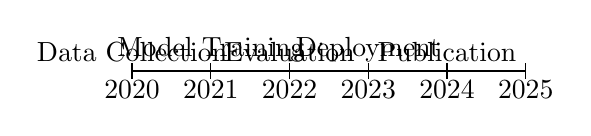
\begin{tikzpicture}[scale=1]
    % Define timeline parameters
    \def\timelineStart{0} % Start of timeline (years)
    \def\timelineEnd{5}   % End of timeline (years)
    
    % Draw timeline line
    \draw[thick] (\timelineStart,0) -- (\timelineEnd,0);
    
    % Place tick marks at each year
    \foreach \x in {0,...,\timelineEnd} {
        \draw (\x,0) node[below] {\the\numexpr\x+2020}; % Label years below line
        \draw (\x,-0.1) -- (\x,0.1); % Tick mark
    }
    
    % Annotate milestones above the line
    \node[above] at (0,0) {Data Collection};
    \node[above] at (1,0) {Model Training};
    \node[above] at (2,0) {Evaluation};
    \node[above] at (3,0) {Deployment};
    \node[above] at (4,0) {Publication};
\end{tikzpicture}
\end{document}